\begin{enumerate}
    %1.
  \item Machine learning is the study of finding or making a function $f$ that takes input $x$(feature vector) from some set $D$ and gives output $y$, where nothing is known about the relationship between $x$ and $y$ a priori.
        Supervised learning is the case where $y$ is known for some subset of $D$.
        Unsupervised learning is the case where nothing is known about the ouput of the function.
        An example would be taking a picture, $x$, of a dog or cat and finding a function, $f$, to classify the picture as a picture of a dog or cat, $y$.
  %2.
  \item
      \begin{enumerate}
        \item Feature scaling is changing the values of (numeric)features so that they conform to some restriction, without significantly changing the information encoded within the features.
        \item Distance based learning algorithms.
          \begin{itemize}
            \item K Nearest Neighbors
            \item Neural networks
          \end{itemize}
        \item Tree based algorithms
          \begin{itemize}
            \item Random forest.
            \item Random forest.
          \end{itemize}
      \end{enumerate}
  %3.
    \item
      \begin{enumerate}
        \item
          \begin{minipage}[t]{0.9\textwidth}
            \centering
            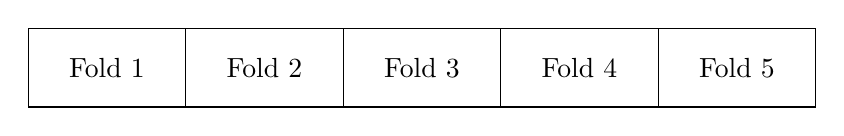
\begin{tikzpicture}[baseline=(current bounding box.north)]
              \draw (0,0) -- (0,1) -- (10,1) -- (10,0) -- (0,0);
              \draw[] (1,0.5) node {Fold 1};
              \draw (2,0) -- (2,1);
              \draw[] (3,0.5) node {Fold 2};
              \draw (4,0) -- (4,1);
              \draw[] (5,0.5) node {Fold 3};
              \draw (6,0) -- (6,1);
              \draw[] (7,0.5) node {Fold 4};
              \draw (8,0) -- (8,1);
              \draw[] (9,0.5) node {Fold 5};
            \end{tikzpicture}
          \end{minipage}
        \item
          \begin{description}
              \item[Advantages] It gives a better estimation of the average generalization of the model.
              \item[Disadvantages] It takes a long time to run.
                                   This is a less significant problem, but more data is generally needed.
          \end{description}
      \end{enumerate}
    \item
      \begin{enumerate}
          \item
            The gradient descent method might only find a local minimum and not the global minimum.
          \item
            By looking at the error data, overfitting of the model can be seen.
            If the model is overfitting then the model is too complex, a lower degree polynomial is required.
            If the model is underfitting the model is too simple and a higher order polynomial is required.

          \item
            By looking at the error data, overfitting of the model can be seen.
            If the model is overfitting then more regularization is needed.
            If the model is starting to underfit then less regularization is needed.
      \end{enumerate}
\end{enumerate}
